 \documentclass[book.tex]{subfiles}
\begin{document}
My personal introduction to computer gaming started in 1985, when my parents bought a MSX-1 Home Computer. I was fascinated by games such as Konami's \textit{Knightmare} and \textit{Nemesis 2}. It was not only the gameplay that interested me, but also how such games are developed. That's how I started my interest into programming and game development.\\
\par
The same year I had my first home computer, Nintendo released a game called \textit{Super Mario Bros.} on the Nintendo Entertainment System (NES). It was an instant blockbuster; it combined great graphics with smooth side scrolling. Side scrolling games from that time period, like Knightmare and Nemesis 2, moved at constant and "choppy" speed. Super Mario Bros. was different, as the player dictates the scrolling speed. You could smoothly accelerate from walk to run or jump, and the screen would smoothly follow your actions. Super Mario Bros. was immensely successful, both commercially and critically. It helped popularize the side-scrolling platform game genre, and served as a killer app for the NES\footnote{Upon release in Japan, 1.2 million copies were sold during its September 1985 release month. Within four months, about 3 million copies were sold in Japan}.\\
\par
Super Mario Bros. showed the real power of the NES, which was hardware supported scrolling. Most computers around that time, like MSX and Commodore-64 computer systems, only had hardware support for sprites. To perform side scrolling on these platforms one  need to move all the background "characters" (typically represented by 8x8 pixel tiles), which is why you get that super choppy "scrolling". The only way to actually get smooth pixel scrolling was by redrawing the entire screen, offset by the number of pixels you want to scroll. This was incredibly performance intensive, and not even possible with most hardware of that time. \\
\begin{figure}[H]
  \centering
 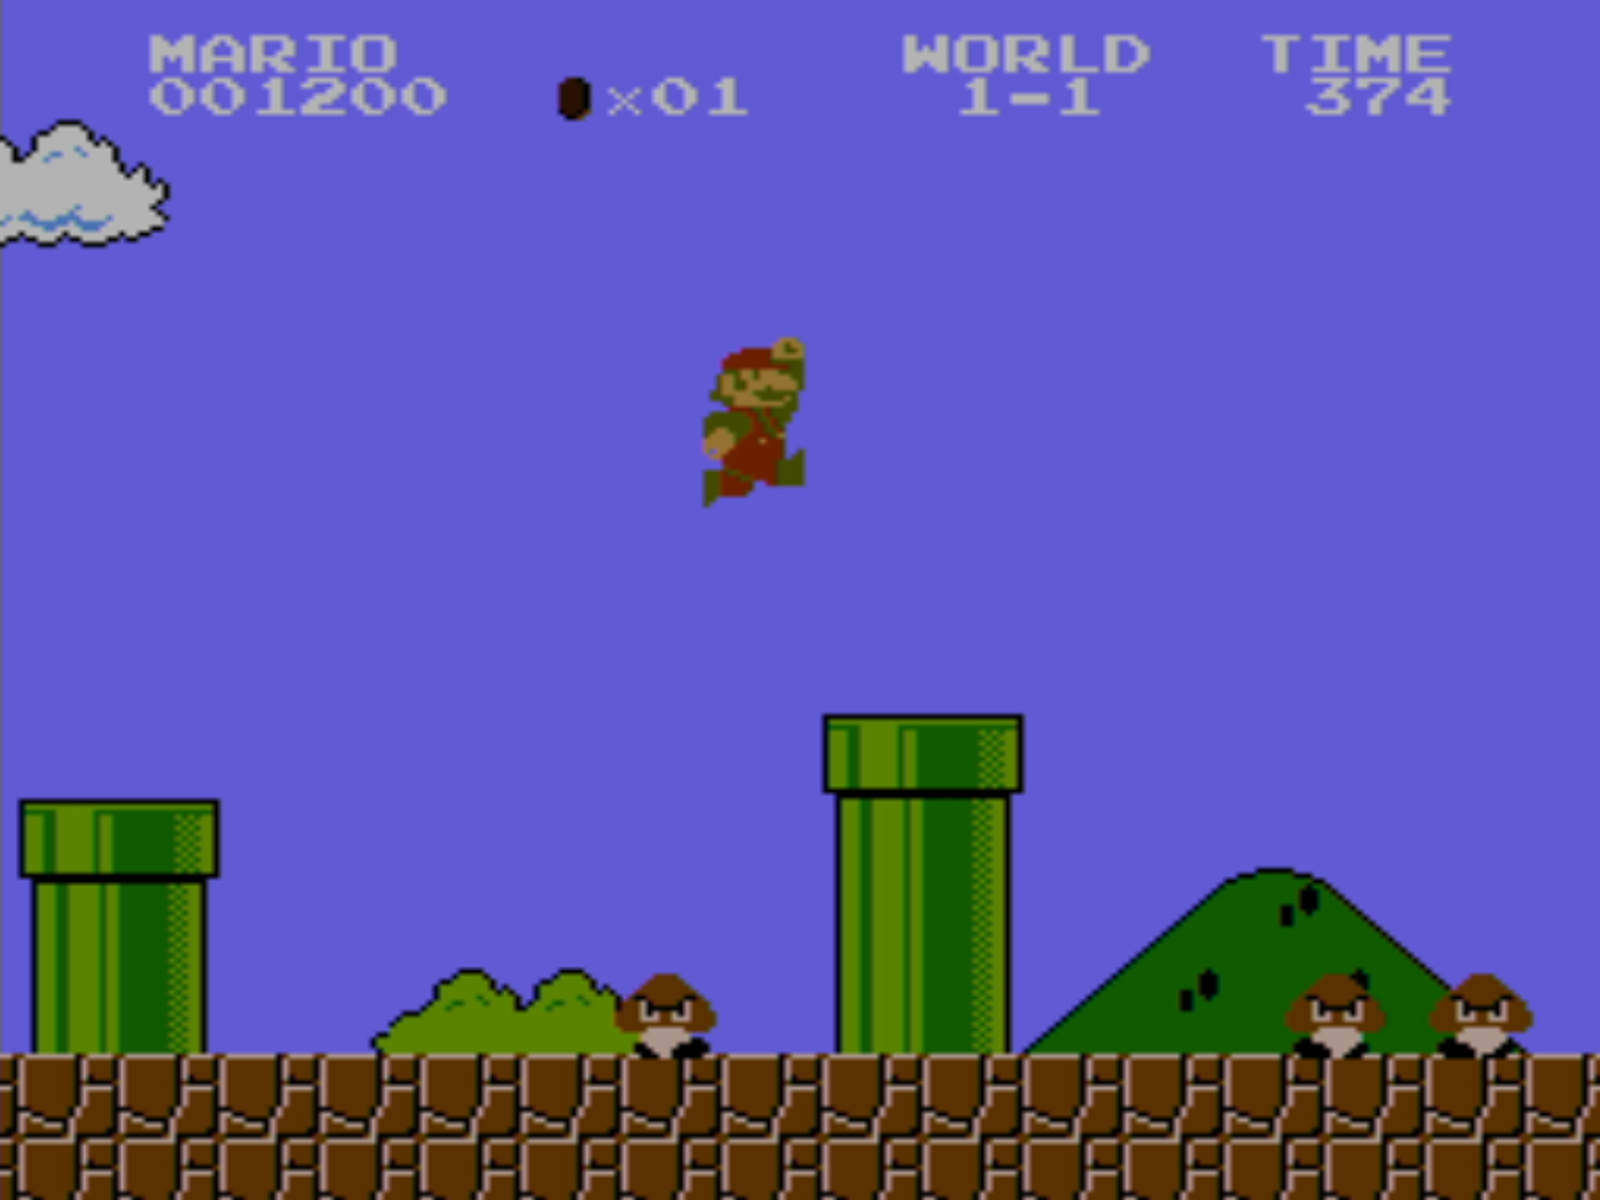
\includegraphics[width=1.0\textwidth]{screenshots_300dpi/Mario_Bros.png}
\caption{Super Mario Bros. on Nintendo Entertainment System}
\end{figure}

\par
The NES was one of the very first home computers that supported smooth scrolling. Essentially, the hardware had a register you could just write to set the fine (pixel) scroll. If you want your background to be displayed scrolled 120 pixels in from the right, and 22 pixels from the top, you just write "120" and then "22" in order, to the same register. Done deal! The video chip takes care of the rest, running at the same constant speed as it always done.\\
\par
The IBM PC was by late 80s far behind the gaming power of the NES. It was designed for office work rather than gaming. It was meant to crunch integers and display static images for word processing and spreadsheet applications. Most PC games around that time are graphic adventure games (King's Quest), static platform games (Prince of Persia) and simulation games (Sim City). Basically, the PC lacked all hardware support for sprites and smooth scrolling.\\
\par
Then, on December 14\textsuperscript{th}, 1990, a small unknown software company called "Ideas from the Deep" released \textit{Commander Keen in Invasion of the Vorticons} for the IBM PC. It was the first smooth side-scrolling game on a PC, similar like Super Mario Bros on the NES. \\
\begin{figure}[H]
  \centering
 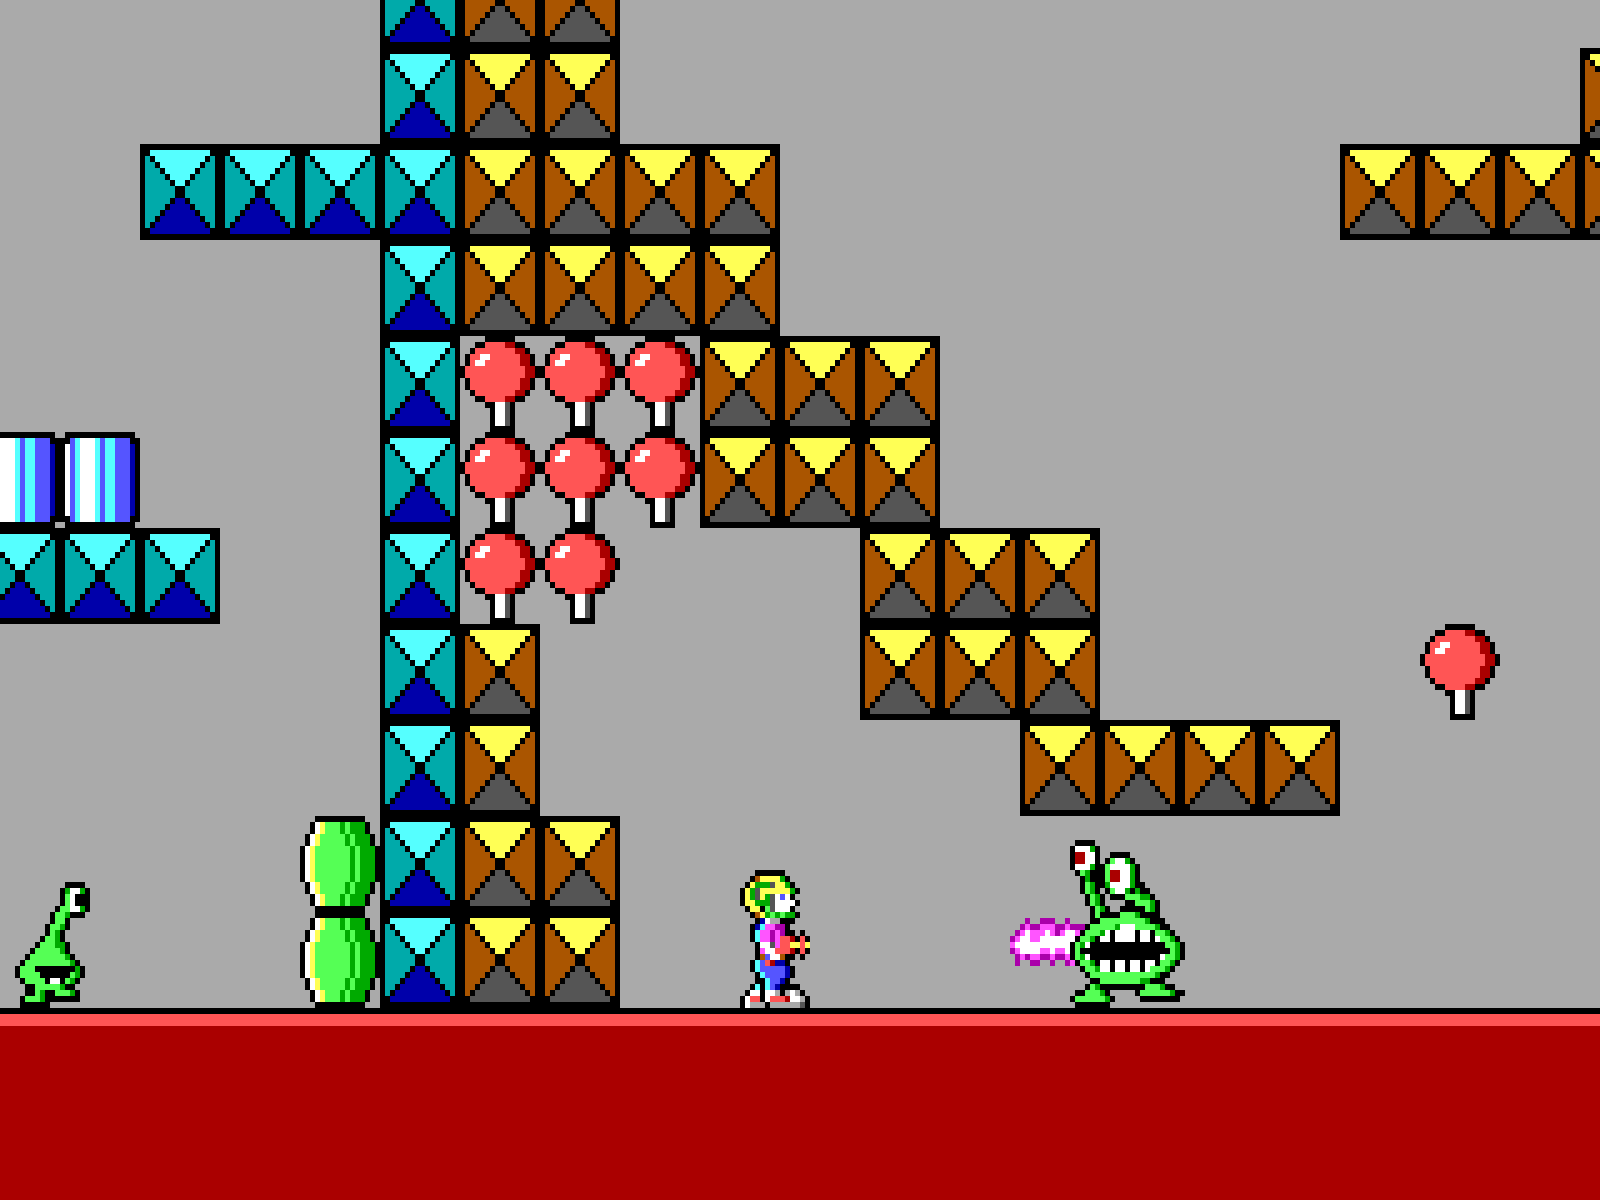
\includegraphics[width=1.0\textwidth]{screenshots_300dpi/Keen_Marooned_on_Mars_gameplay.png}
\caption{Commander Keen in Invasion of the Vorticons}
\end{figure}
\par

How was this possible on the IBM PC? Many obstacles had to be overcome:
\begin{itemize}
  \item The first 8086 CPU did not outperform the average home computer in terms of raw power. Only with the release of the 286 CPU the PC started to outperform the market in terms of raw power.
  \item As stated before, the video system (called EGA) did not support any form of scrolling. It did not even support any form of sprites, which allowed movement of something on the screen by simply updating its \cw{(x,y)} coordinates.
  \item The video system could not double buffer. It was not possible to have smooth scrolling without ugly artifacts called "tears" on the screen.
  \item The PC Speaker, the default sound device, could only produce square waves resulting in a bunch of "beeps" which were more annoying than anything else.
  \item The audio ecosystem was fragmented. Each of the various sound systems had
different capabilities and expectations
  \item The RAM addressing mode was not flat but segmented, resulting in complex and
error prone pointer arithmetic.
  \item The bus was slow and I/O with the VRAM was a bottleneck. It was next to impossible to write a full framebuffer at 70 frames per second
\end{itemize}
\par

\begin{figure}[H]
\centering
  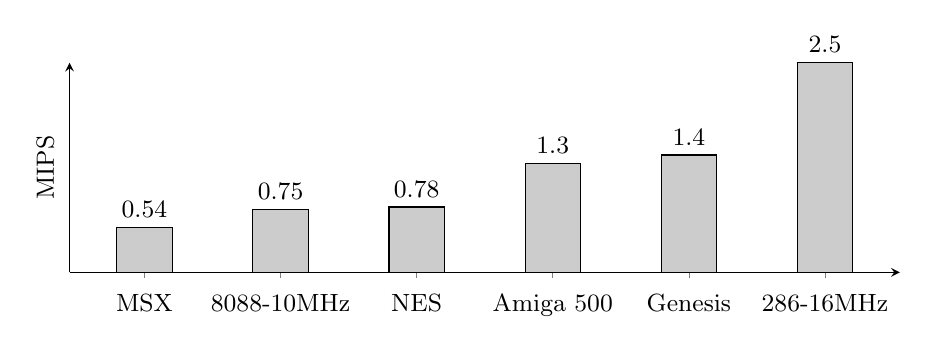
\begin{tikzpicture}[font=\small]
    \begin{axis}[
      width=\textwidth,
      height=0.35\textwidth,
      ybar=6pt,
      bar width=20pt,
      ylabel={MIPS},
      ymin=0,
      ytick=\empty,
      xtick=data,
      axis x line=bottom,
      axis y line=left,
      enlarge x limits=0.11,
      symbolic x coords={MSX, 8088-10MHz, NES, Amiga 500, Genesis, 286-16MHz},
      xticklabel style={anchor=base,yshift=-\baselineskip},
      nodes near coords={\pgfmathprintnumber\pgfplotspointmeta}
    ]
      \addplot[fill=black!20,draw=black] coordinates {
        (MSX, 0.54)
        (8088-10MHz, 0.75)
        (NES, 0.78)
        (Amiga 500,1.3)
        (Genesis,1.4)
        (286-16MHz, 2.5)
      };
    \end{axis}
   \end{tikzpicture}
   \caption{Consoles\protect\footnotemark vs PC, CPU comparison with MIPS\protect\footnotemark\protect\footnotemark.}
   \label{fig:ems_xms_layout}
 \end{figure}
 % Latex footnote I HATE YOU !!!!!!
 \addtocounter{footnote}{-2}
 \footnotetext{The MSX uses a Zilog Z80 running at 3.6MHz. The Amiga 500 and Genesis have a Motorola 68000 CPU respectively running at 7.16 MHz and 7.6 MHz. The NES uses a Ricoh 2A03 CPU running at 1.8 MHz.}
 \stepcounter{footnote}
 \footnotetext{Million Instructions Per Second.}
 \stepcounter{footnote}
 \footnotetext{Gamicus Fandom: https://gamicus.fandom.com/wiki/Instructions\_per\_second.}


Overall, it seemed impossible to create any reasonable side-scrolling game on the PC platform. But many around the world did not accept that and tinkered with the hardware to achieve unexpected results. How they did it is the \textit{raison d'\^etre} of this book. I've chosen to divide this book into four chapters:
\begin{itemize}
  \item Chapter 2: The Hardware. The five components of a PC from 1990.
  \item Chapter 3: The tools and assets. Which tools are used for game development and how are assets created and structured.
  \item Chapter 4: The Software. The Commander Keen game engine.
  \item Chapter 5: Commander Keen game engine in CGA graphics.
\end{itemize}
By first showing the hardware constraints, I hope programmers will develop an appreciation for the software and how it navigated obstacles, sometimes turning limitations into advantages.\\
\par
The book is based on \textit{Commander Keen in Keen Dreams}, which is developed after the first 3 releases of the game. The reason is that this is the only version where the source code is publicly released. Where needed, I will also explain how the technology changed between the different versions of Commander Keen, but it will be without code examples unfortunately.\\
\begin{figure}[H]
  \centering
 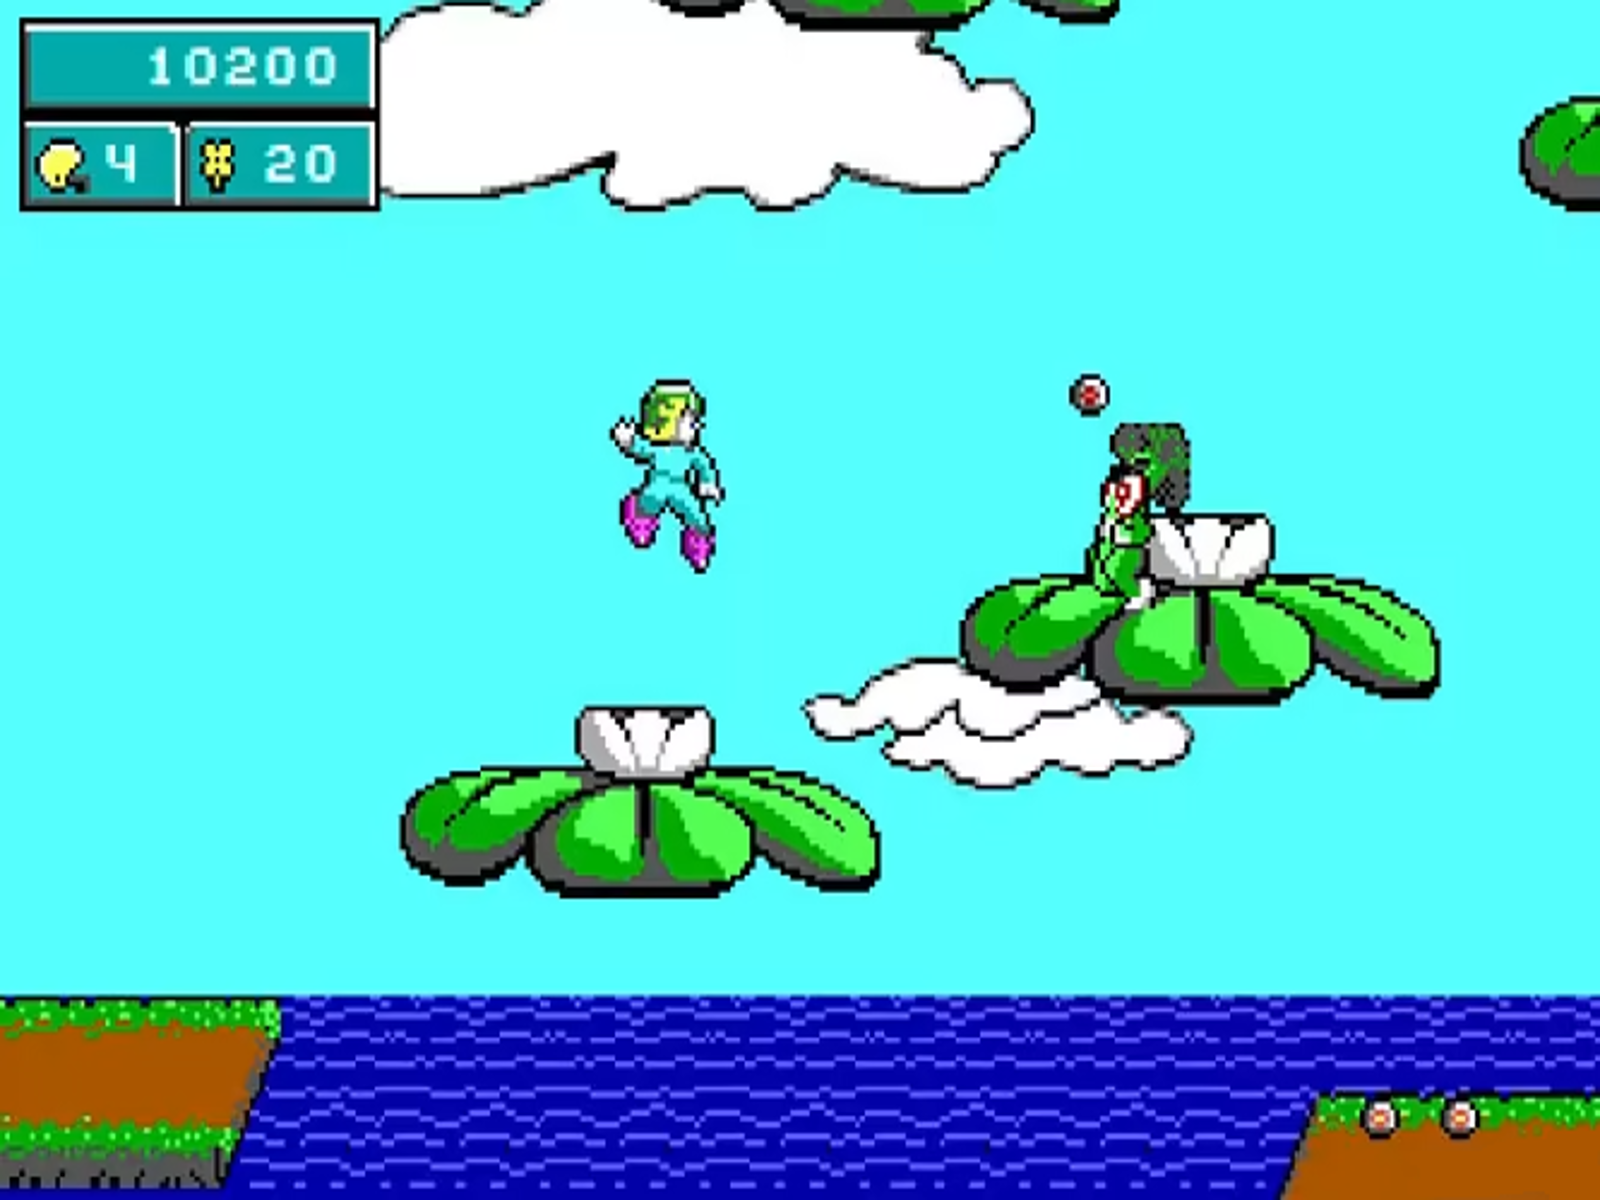
\includegraphics[width=1.0\textwidth]{screenshots_300dpi/Keen_Dreams.png}
\caption{Commander Keen in Keen Dreams}
\end{figure}
\par






\end{document}